\documentclass[11pt,a4paper]{article}
\usepackage[margin=22mm]{geometry}
\usepackage{fontspec}\setmainfont{STIXGeneral}
\usepackage{amsmath,booktabs,array,graphicx,xcolor,hyperref}
\hypersetup{colorlinks=true,linkcolor=blue,urlcolor=blue}
\setlength{\parindent}{0pt}\setlength{\parskip}{5pt}
\newcommand{\smalltable}{\small\setlength{\tabcolsep}{5pt}\renewcommand{\arraystretch}{1.13}}
\begin{document}
\begin{center}\Large\textbf{Ten topics: complete papers and conditional applications}\end{center}
This report brings together the accepted measurements for \textbf{27 distinct original manuscripts} in ten canonical topics. It does not complete the 161-item registry. The later accepted F015 and L028 contracts are not yet measured and are outside this fixed numerical baseline. The task is to derive the specified main results from complete common theories and applications, with corrections, retained outside theorems and exclusions recorded in each scientific admission. No new mathematical result or source credit is asserted here.

For topic $T$, write $S_T=\sum_i c(L_i)$ for the full original manuscripts, $U_T=c(U)$ for the entire common paper, and $A_T=\sum_i c(A_i)$ for all complete applications. The two headline comparisons are
\[
 R_T=\frac{S_T}{U_T+A_T},\qquad
 r_{T,i}=\frac{c(L_i)}{c(A_i)}\quad
 \text{after acquiring all of $U$ and the declared programs.}
\]
Every topic pays its own whole common theory even when another topic contains overlapping mathematics. A factor above one means fewer measured characters in the replacement; a factor below one means more. The conditional factors do not describe a complete replacement obtained at the cost of the application alone.

\textbf{Complete written papers.} Costs below are NFC characters without whitespace, at each topic's accepted primary representation. They include introductions, definitions, proof text and references as prescribed by the fixed input boundaries.
\begin{center}\smalltable
\begin{tabular}{lrrrrrr}\toprule
Topic & Originals & Sources & Common & Applications & Ours & Factor\\\midrule
A & 6 & 195,379 & 49,059 & 78,251 & 127,310 & 1.535 \\
B$^*$ & 4 & 73,012 & 14,124 & 44,959 & 59,083 & 1.236 \\
C$^*$ & 4 & 73,953 & 27,142 & 44,163 & 71,305 & 1.037 \\
D & 3 & 47,894 & 15,632 & 29,855 & 45,487 & 1.053 \\
E & 3 & 71,375 & 19,790 & 19,513 & 39,303 & 1.816 \\
F & 1 & 25,115 & 7,118 & 12,744 & 19,862 & 1.264 \\
G & 2 & 73,199 & 30,928 & 85,207 & 116,135 & 0.630 \\
Affine & 1 & 32,767 & 19,070 & 22,638 & 41,708 & 0.786 \\
Represent. & 1 & 25,348 & 11,288 & 13,688 & 24,976 & 1.015 \\
Chamber & 2 & 35,802 & 15,199 & 21,254 & 36,453 & 0.982 \\
\bottomrule\end{tabular}\end{center}
\textbf{Representation matters.} Unstarred rows use the accepted full selected PDF text with calibrated glyphs and recorded page furniture excluded. In B and C, N001 and L108 are complete literal text renderings; every other source and every replacement PDF in those two comparisons is counted \emph{untrimmed}. No speculative symbol repair is made to the rendered bodies. Their original PDF costs remain unknown in the earlier PDF records. These two representations are not pooled into a programme-wide factor.

The full-source numerator concerns the agreed principal results, not every ancillary assertion. Retained external proofs, unknown historical software, full image/layout information and end-to-end formalization have no invented zero cost. The tables measure documents under the admitted boundaries, not an absolute minimum proof complexity.
\newpage
\textbf{Whole-topic written costs.} Each dark bar is the complete source sum. The paired bar pays the entire common theory (blue) and all complete applications (green). Both bars use the same scale. The separate representations for B and C remain explicit.
\begin{center}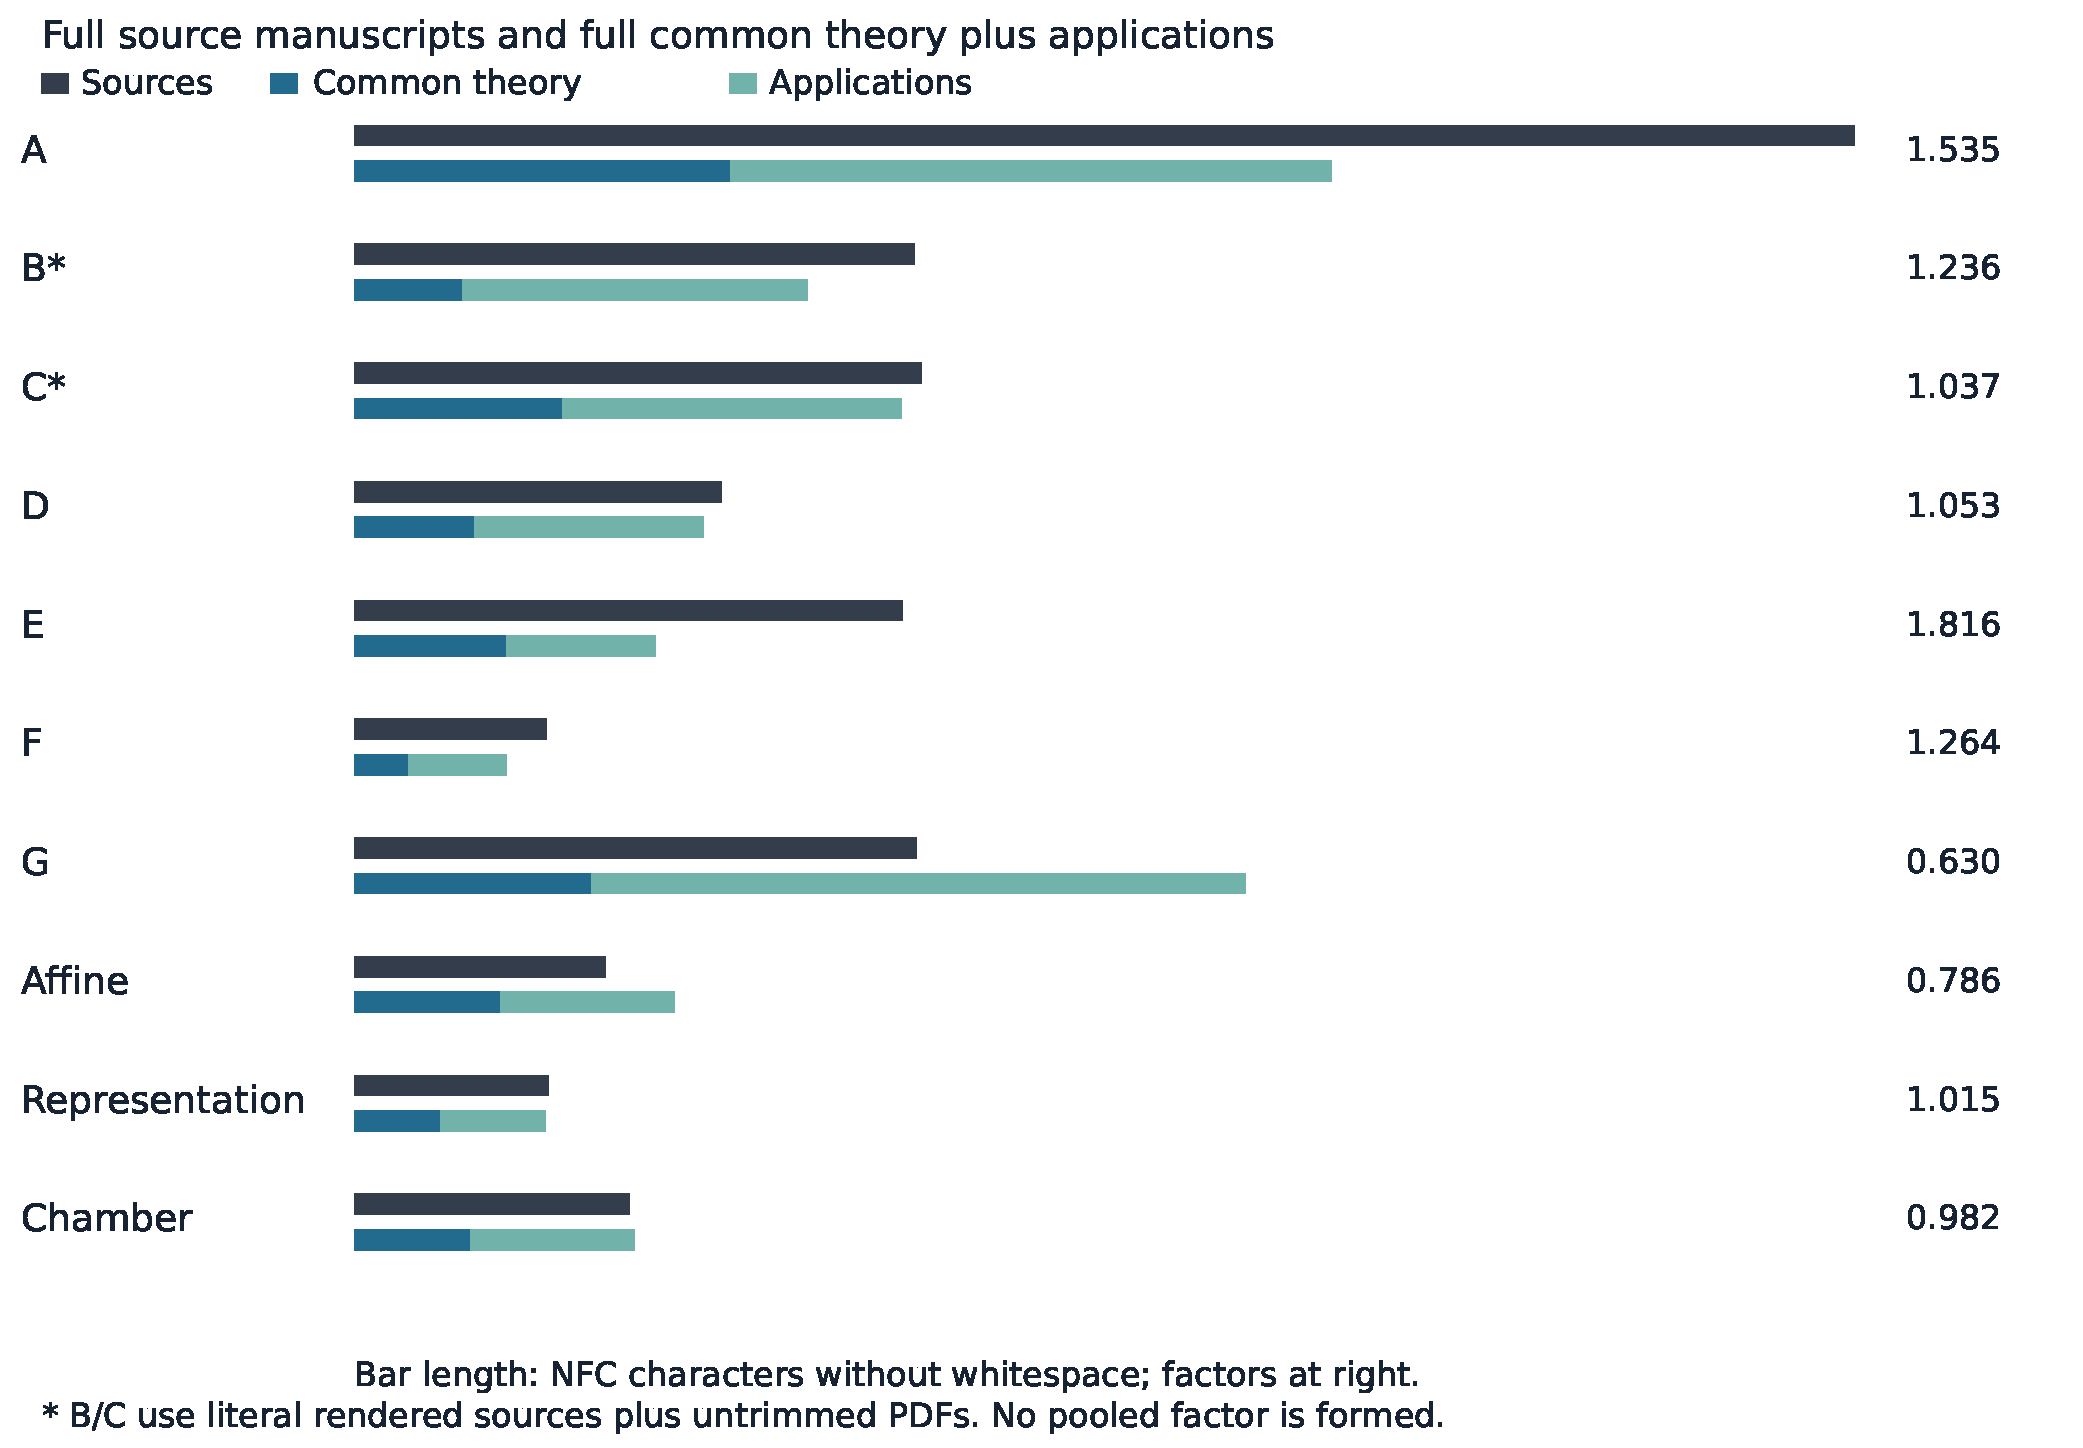
\includegraphics[width=\linewidth]{whole_topics.pdf}\end{center}
The displayed factors retain cases that do not shorten the written record: Affine, G and Chamber are longer overall in this coordinate. Small factors above one also require the stated unit: for Representation, the admitted calibrated UTF-8 comparison is approximately $0.970886$, rather than above one. Other units and boundary sensitivities remain available in the underlying packets; this report does not select a different favourable coordinate for each row.

G includes the L009 publisher cover in its primary numerator; its article-only alternative is separate. E uses its current readable edition, with the added motivation and clarifications charged in full. No earlier, shorter language edition is substituted.
\newpage
\textbf{Complete programs and prior acquisition.} The following alternatives add the entire declared printed program appendix to the written denominator, or replace that appendix by the cost of its whole raw files. Printed and raw versions are never both charged. These costs include different roles, made explicit below; validations are not silently described as mathematical premises.
\begin{center}\smalltable
\begin{tabular}{lrrrrr}\toprule
Topic & Printed code & With printed & Raw alternative & With raw & $U+$printed\\\midrule
A & 53,035 & 1.083 & 51,970 & 1.090 & 102,094 \\
B$^*$ & 0 & 1.236 & 0 & 1.236 & 14,124 \\
C$^*$ & 8,803 & 0.923 & 8,323 & 0.929 & 35,945 \\
D & 27,070 & 0.660 & 26,185 & 0.668 & 42,702 \\
E & 7,565 & 1.523 & -- & -- & 27,355 \\
F & 8,837 & 0.875 & 8,061 & 0.899 & 15,955 \\
G & 53,018 & 0.433 & 50,184 & 0.440 & 83,946 \\
Affine & 17,250 & 0.556 & 16,682 & 0.561 & 36,320 \\
Represent. & 9,025 & 0.746 & 8,310 & 0.762 & 20,313 \\
Chamber & 7,677 & 0.811 & 6,401 & 0.835 & 22,876 \\
\bottomrule\end{tabular}\end{center}
The final column is the full prepaid amount for every conditional row on the next page. B has no required mathematical program in its complete written contract. E's optional validation file adds a further 5,173 characters; including it gives factor $1.372$. E's raw alternative is not introduced here because it was not an admitted headline coordinate.

\begin{itemize}\setlength\itemsep{1pt}
\item A: four complete files in the admitted code, data and runner appendix; C: two required GAP programs; Affine: six required mathematical programs.
\item D: five required programs and three diagnostics. G: four required finite computations, two programs for witnesses and certificates, and seven validations. Chamber: one required GAP program and one diagnostic.
\item E: one required GAP program, with one optional validation program shown separately. F: three validation programs and no uniform finite proof premise. Representation: two validation programs and no uniform finite proof premise.
\end{itemize}
Other operational drivers and partial Lean evidence remain separately inventoried in the underlying admissions. Their absence from a written-paper denominator is explicit, not a claim that execution, verification or full formalization is free. The programme comparison is conditioned on the named retained mathematical inputs; their full proof costs remain unknown. No claim about a historical software cost follows from its absence from a supplied manuscript.

\textbf{Mathematical interpretation.} Each common paper is charged once within its topic. Every application retains its complete local proof obligations. A short application can therefore express a substantial consequence after common theory has been established; it does not establish historical novelty of that common theory. Attribution and corrected source claims remain governed by the accepted source maps.
\newpage
\textbf{Every original and its complete application.} These are conditional comparisons after the full acquisition shown on the previous page. E1--E3 are display names for the admitted files New\_A1--New\_A3. No application or original is omitted because its factor is below one.
\begin{center}\smalltable
\begin{tabular}{lllrrr}\toprule
Topic & Original & Application & Original cost & Application cost & Conditional\\\midrule
A & L032 & A1 & 16,558 & 8,212 & 2.016 \\
A & L034 & A2 & 21,433 & 5,784 & 3.706 \\
A & F016 & A3 & 43,983 & 15,419 & 2.853 \\
A & F013 & A4 & 25,562 & 6,224 & 4.107 \\
A & L035 & A5 & 51,019 & 14,498 & 3.519 \\
A & N009 & A6 & 36,824 & 28,114 & 1.310 \\
B$^*$ & N001 & B1 & 14,519 & 7,371 & 1.970 \\
B$^*$ & N003 & B2 & 17,780 & 14,170 & 1.255 \\
B$^*$ & N008 & B3 & 18,009 & 11,132 & 1.618 \\
B$^*$ & L030 & B4 & 22,704 & 12,286 & 1.848 \\
C$^*$ & L088 & C1 & 13,166 & 11,311 & 1.164 \\
C$^*$ & N013 & C2 & 27,361 & 15,815 & 1.730 \\
C$^*$ & L108 & C3 & 12,849 & 10,075 & 1.275 \\
C$^*$ & F014 & C4 & 20,577 & 6,962 & 2.956 \\
D & L066 & D1 & 20,916 & 10,989 & 1.903 \\
D & L074 & D2 & 20,661 & 13,367 & 1.546 \\
D & L104 & D3 & 6,317 & 5,499 & 1.149 \\
E & L083 & E1 & 20,885 & 3,002 & 6.957 \\
E & L079 & E2 & 20,908 & 1,855 & 11.271 \\
E & L021 & E3 & 29,582 & 14,656 & 2.018 \\
F & L014 & F1 & 25,115 & 12,744 & 1.971 \\
G & L009 & G1 & 49,891 & 23,544 & 2.119 \\
G & L092 & G2 & 23,308 & 61,663 & 0.378 \\
Affine & L012 & AF1 & 32,767 & 22,638 & 1.447 \\
Represent. & F010 & R1 & 25,348 & 13,688 & 1.852 \\
Chamber & L008 & H1 & 21,784 & 7,571 & 2.877 \\
Chamber & N016 & H2 & 14,018 & 13,683 & 1.024 \\
\bottomrule\end{tabular}\end{center}
The original identifiers are unique across these ten topics. The machine-readable companion supplies exact fractions, all input hashes and the full source/application lists. The existing topic packets preserve all measured units and sensitivities. This consolidation changes no proof, source boundary, conjecture status or existing numerical input.
\newpage
\textbf{Application costs after common theory acquisition.} Dark bars show complete originals; green bars show complete applications. The full common theory and declared programs have already been acquired independently for each topic. The bars measure text cost, not theorem counts.
\begin{center}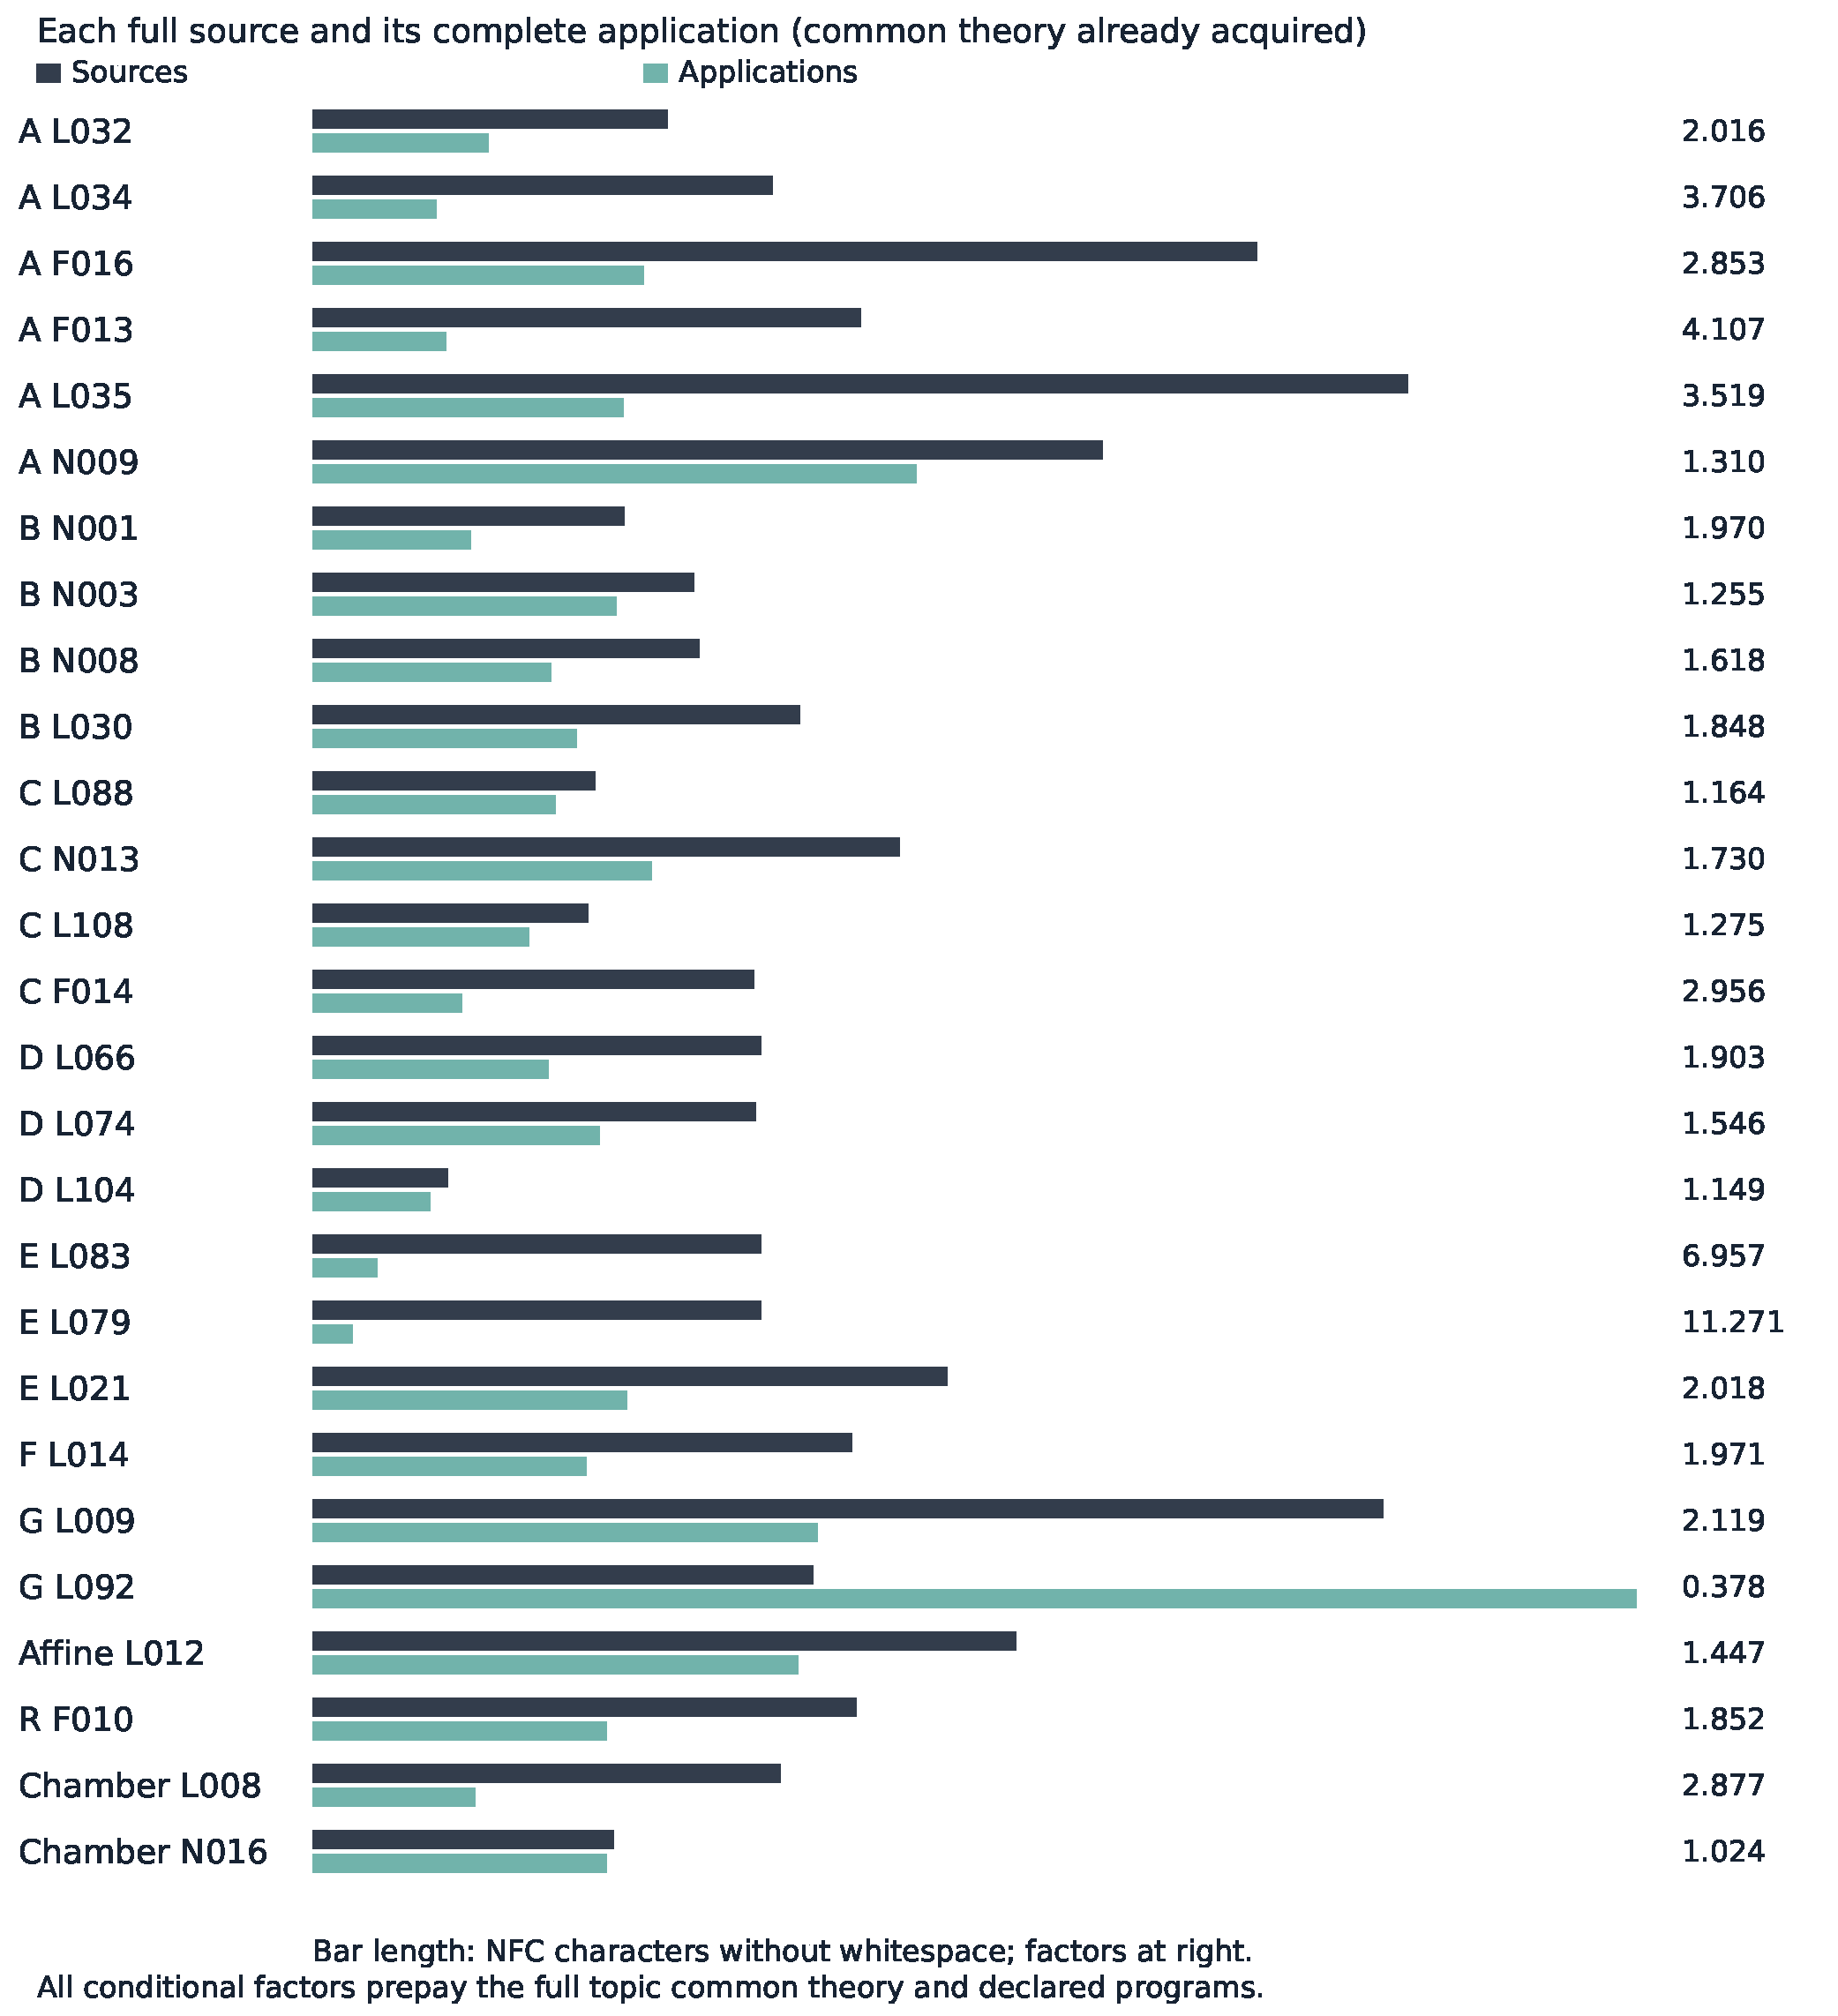
\includegraphics[width=\linewidth,height=0.82\textheight,keepaspectratio]{conditional_applications.pdf}\end{center}
\end{document}
